\section{Background: the paradox and its diagnosis}
\label{sec:background}

This section recaps the result this paper extends \citep{anon-workshop}. All
numbers here are reproductions on our own runs; the claims are prior work.

\subsection{Question-first perceives better and answers worse}

Table~\ref{tab:ladder} runs six orderings on four benchmarks with Qwen3-VL-8B.
Every column uses the same system message, question string, image, decoding and
scoring code; \sti{} and \sit{} contain the same tokens in the same quantity.
Only the position of the question moves. Question-first is the worst ordering on
all four: NaturalBench group accuracy falls from $35.05$ to $26.95$
($p = 1.3\times10^{-12}$), Winoground from $31.75$ to $22.25$
($p = 7.7\times10^{-5}$), RF20 F1 from $78.57$ to $65.59$.

The obvious explanation, that question-first degrades perception, is wrong.
Reading image patches with a logit lens, question-first makes $6.975$ patches
per image decode a question content word against $2.800$ for question-last, a
factor of $2.49$ over 160 NaturalBench candidates. Figure~\ref{fig:steering}
shows this patch by patch: asking ``Is the adult in the image chasing a child?''
before the image turns \emph{running} into \emph{chase}, \emph{boy} into
\emph{ahead} and \emph{baseball} into \emph{child}, taking the count of patches
decoding a question word from 1 to 12, and the model then answers ``No'' to a
question whose ground truth is Yes.

\begin{table}[t]
\caption{Ordering ladder on four benchmarks, Qwen3-VL-8B, reproducing
\citet{anon-workshop} and adding RF20. \sti{} (question first) is worst
everywhere. POPE is the exception to the repair: plain question-last already
wins there. $N$: NaturalBench 1{,}900 groups, POPE 9{,}000, Winoground 400
examples, RF20 24{,}449.}
\label{tab:ladder}
\begin{center}
\small
\begin{tabular}{llrrrrrr}
\toprule
Benchmark & Metric & \ist{} & \sit{} & \sti{} & \stit{} & \sitit{} & \sititrev{} \\
\midrule
NaturalBench & pair acc.  & 78.93 & 79.21 & 75.29 & 78.95 & \best{80.36} & 80.26 \\
NaturalBench & group acc. & 33.95 & 35.05 & 26.95 & 35.00 & \best{37.37} & \best{37.37} \\
POPE         & F1         & 88.22 & \best{88.35} & 86.13 & 87.61 & 88.12 & 88.25 \\
Winoground   & group acc. & 28.00 & 31.75 & 22.25 & 37.50 & 40.25 & \best{41.00} \\
RF20         & F1         & 78.92 & 78.57 & 65.59 & 78.61 & \best{80.56} & 79.78 \\
\bottomrule
\end{tabular}
\end{center}
\end{table}

\begin{figure}[t]
\begin{center}
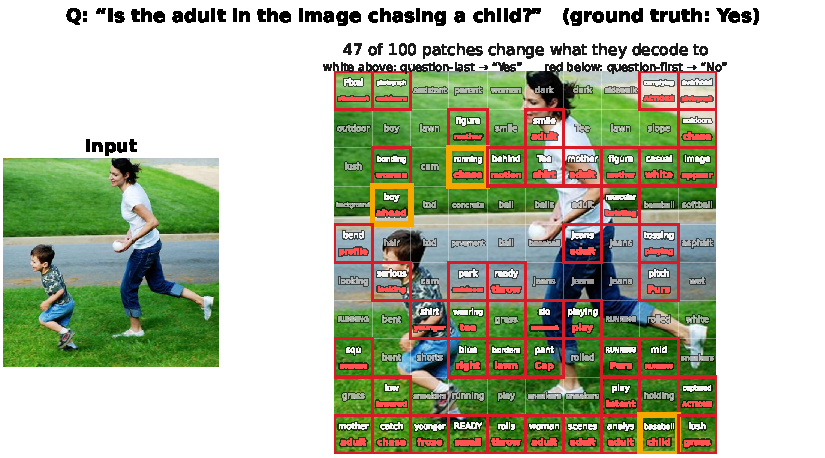
\includegraphics[width=\linewidth]{figs/fig1_chase.pdf}
\end{center}
\caption{Steering happens, and is not read out. Every image patch is shown:
each cell holds the vocabulary token that patch's layer-32 hidden state decodes
to under the logit lens, shaded by that token's probability. Red rings mark
patches decoding a word from the question. Question-last leaves the patches
generic (1 ringed patch) and answers correctly; question-first steers the same
patches onto the question's vocabulary (12 ringed patches) and answers wrong.
Dashed arrows trace three individual patches from question-last to
question-first, ringing each patch at both ends, where \emph{running} becomes
\emph{chase}, \emph{boy} becomes \emph{ahead}, and \emph{baseball} becomes
\emph{child}. Echoing the question keeps all 12 steered patches and answers
correctly again.}
\label{fig:steering}
\end{figure}

\subsection{The failure is read-out, and it is causal}
\label{sec:background-readout}

Probing the answer position on the $150$ NaturalBench pairs where question-first
is wrong and question-last is right, question-first sends $2.19\times$ less
attention to the question at the peak read-out layer ($0.0676$ vs $0.1479$) and
over twice as much to the image. The two orderings are indistinguishable at
chance through layer 25 of 36, then fork at layer 26 and reach
$P(\text{correct})$ of $0.0986$ and $0.8747$ (Figure~\ref{fig:mechanism}).

An attention knockout makes the dependence causal and doubly dissociated
(Appendix~\ref{app:knockout}): severing answer-to-question costs question-last
$5.6$ points (95\% CI $[+1.99, +9.60]$) and question-first nothing ($+0.4$),
while severing answer-to-image costs question-first $9.6$ points and
question-last nothing. An equal-length random span moves both by at most $0.8$.

\begin{figure}[t]
\begin{center}
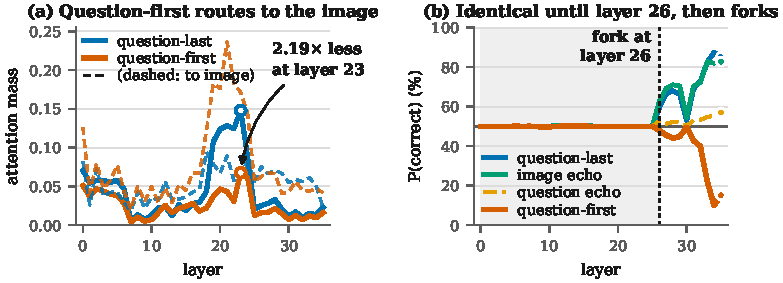
\includegraphics[width=\linewidth]{figs/fig_mechanism.pdf}
\end{center}
\caption{Where question-first breaks (150 NaturalBench pairs where it is wrong
and question-last is right). \textbf{(a)} Attention leaving the answer position,
to the question (solid) and the image (dashed): at layer 23 question-first sends
$2.19\times$ less to the question. \textbf{(b)} $P(\text{correct})$ per layer.
The two baselines sit at chance through layer 25, fork at 26 and never re-cross;
both echo orderings track question-last.}
\label{fig:mechanism}
\end{figure}

\subsection{The repair, and what it leaves open}

The diagnosis prescribes the prompt: if the answer position cannot read the
question, put something after the image that it can read. Question echoing
(\stit{}) repeats the question after the image, which restores question-answer
adjacency while provably leaving perception untouched, since causal masking
means a later copy cannot alter earlier patches
($\cos(\sti{}, \stit{}) = 0.99999$). Image echoing (\sitit{}) repeats the image
after the question. Prior work also showed that reversing the echoed copy
(\sititrev{}) changes little, which we reproduce: NaturalBench group accuracy
moves from $37.37$ to $37.37$ ($p = 1.00$) and Winoground from $40.25$ to
$41.00$ ($p = 0.68$).

That work listed the second image's token cost as an open limitation and did not
measure it. Sections~\ref{sec:generality} to~\ref{sec:gepa} take up that thread:
what the echo costs, how little of it is needed, where the repair stops working,
and whether a prompt optimizer would find it anyway.
